%=============================================================================
%   Configurations Found
%   Reporte de pentominos - Experiment Results
%   Servicio social - Laura Natalia Borbolla Palacios
%=============================================================================

\newpage
\subsection{Configurations found}
\label{sec:configurations-found}
Below are presented the configurations that were found while observing the
evolutions of the pentominoes; it is important to remark that, due to the
fast-paced population growth in some pentominoes, it is possible that some
configurations remain hidden. The configurations are listed in the order that
they were found.

\subsubsection{Gliders}

For more information, please consult \cite{j2}.

The gliders, as explained in section \ref{sec:brief_summary:cellular_automaton},
are mobile particles traveling in the space. There are two types of gliders:
primary and compound; the first ones cannot be decomposed into smaller mobile
localizations, whereas a compound glider is made of at least two primary
gliders. Some properties of the gliders are listed below:
\begin{itemize}
  \item Volume
  \item Translation
  \item Period
  \item Speed
  \item Weight
\end{itemize}

One of the primary gliders in the Diffusion Rule is shown in
figure~\ref{fig:dr-glider-1}.

\begin{figure}
	\centering
	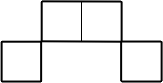
\includegraphics[scale=0.5]{df_settings_dd/dr-glider-1.png}
	\caption{G1 glider in the Diffusion Rule.}
  \label{fig:dr-glider-1}
\end{figure}

\begin{figure}
	\centering
	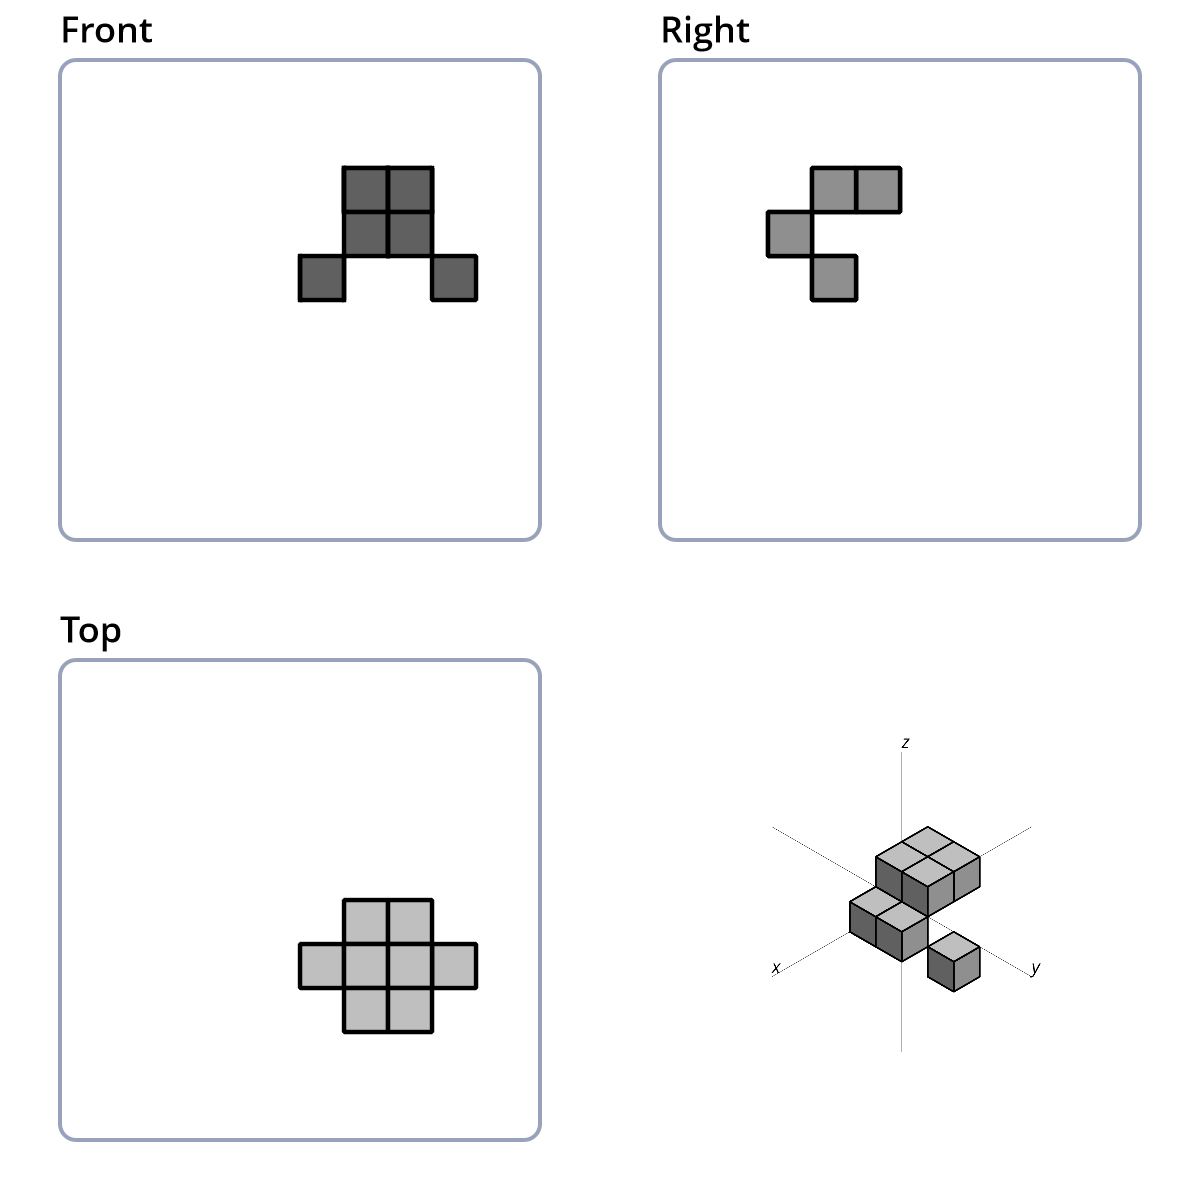
\includegraphics[scale=0.4]{iso_settings/glider_1.png}
	\caption{Isometric of glider-1.}
  \label{fig:iso-glider-1}
\end{figure}

\begin{figure}
	\centering
	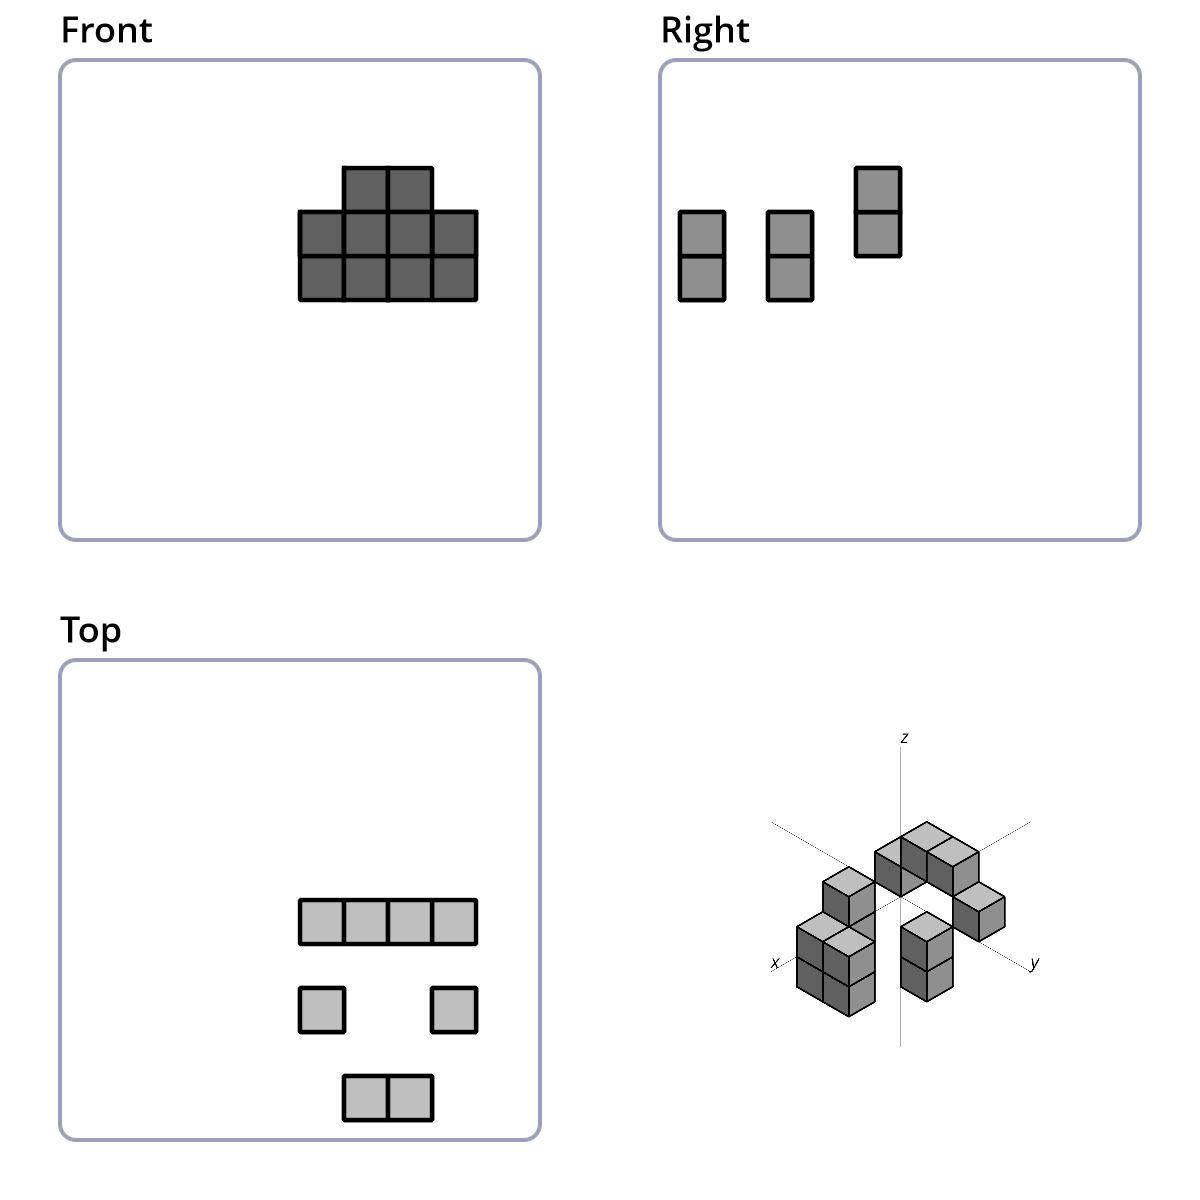
\includegraphics[scale=0.4]{iso_settings/glider_2.png}
	\caption{Isometric of glider-2.}
  \label{fig:iso-glider-2}
\end{figure}

\begin{figure}
  \centering
  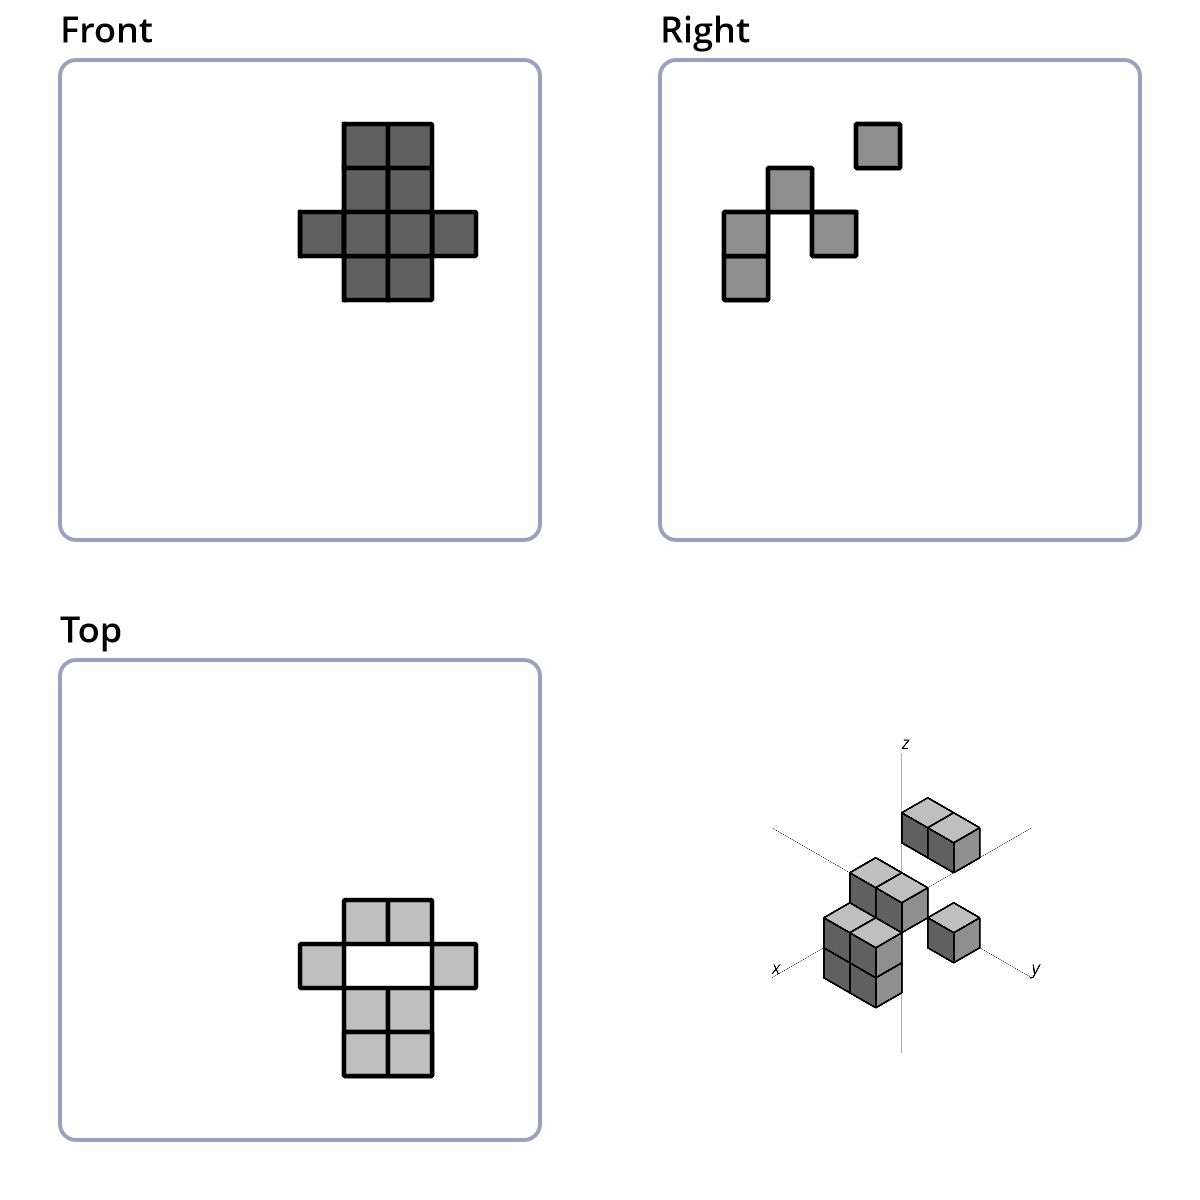
\includegraphics[scale=0.4]{iso_settings/glider_3.png}
  \caption{Isometric of glider-3.}
  \label{fig:iso-glider-3}
\end{figure}

The glider-4 (see figure~\ref{fig:iso-glider-4}) probably is the most simple
glider; the equivalent of G1 (see figure~\ref{fig:dr-glider-1}) in three
dimensions.

\begin{figure}
  \centering
  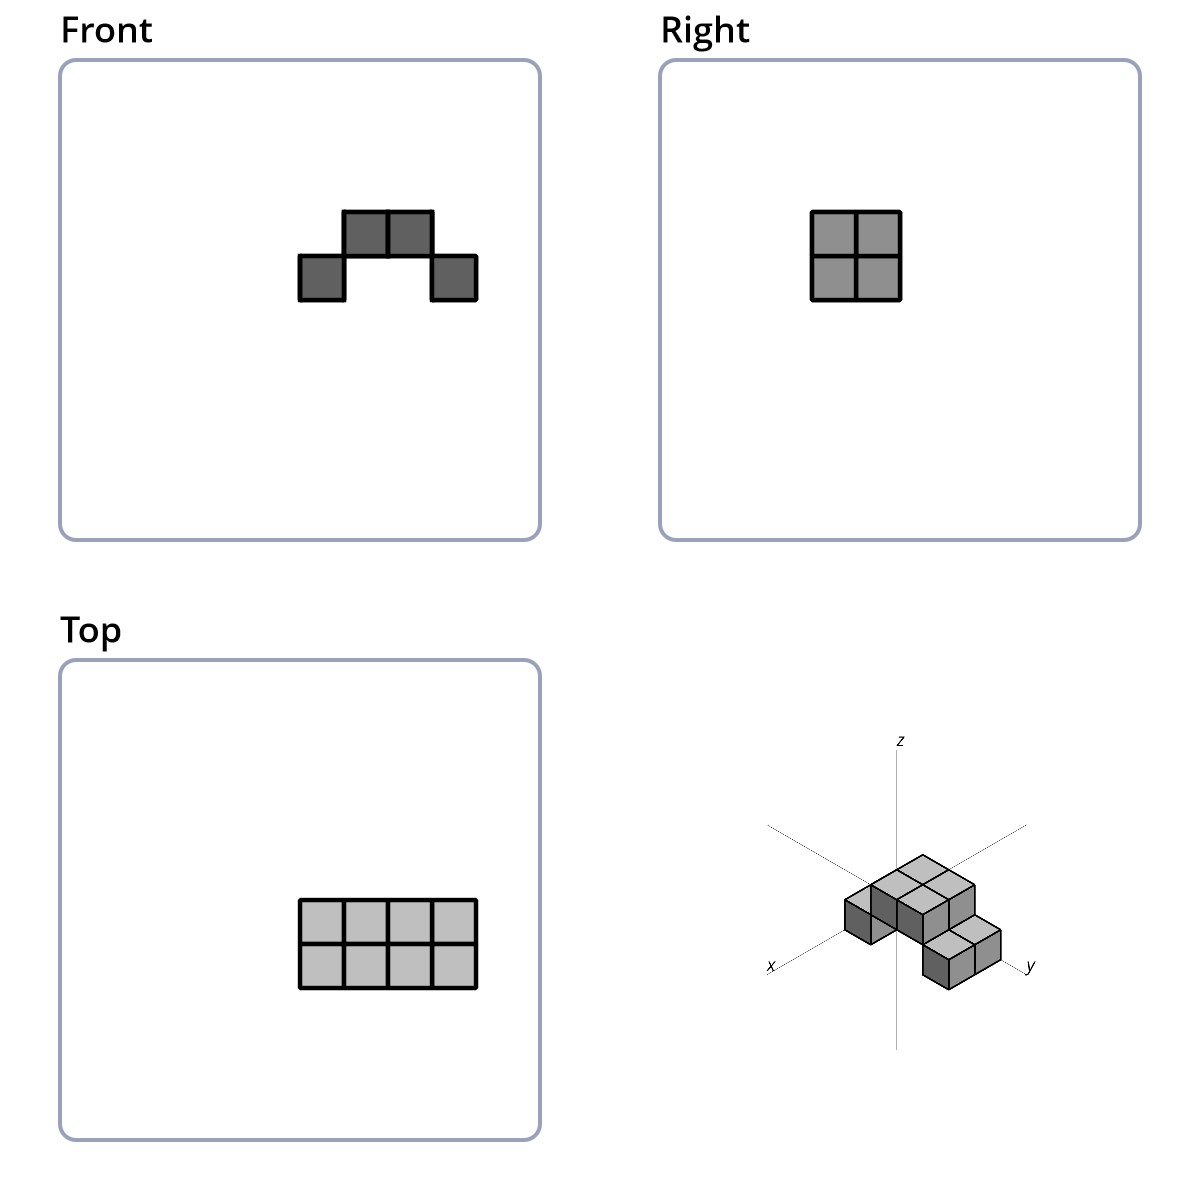
\includegraphics[scale=0.4]{iso_settings/glider_4.png}
  \caption{Isometric of glider-4.}
  \label{fig:iso-glider-4}
\end{figure}


\subsubsection{Oscillators}

\begin{figure}
	\centering
	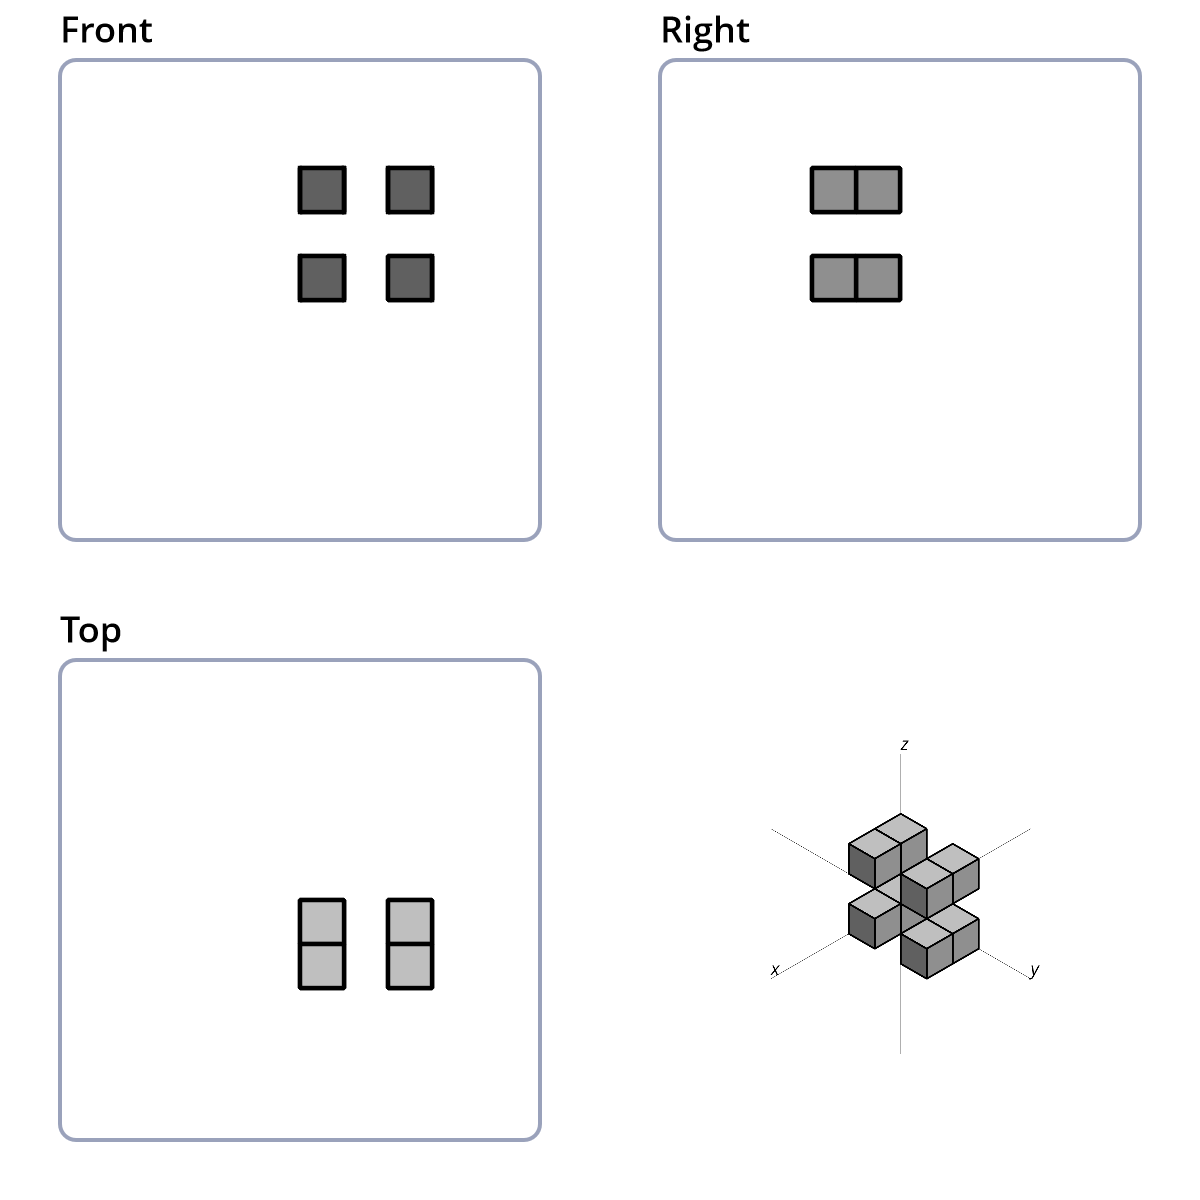
\includegraphics[scale=0.4]{iso_settings/osc_1.png}
	\caption{Isometric of oscillator-1.}
  \label{fig:iso-osc-1}
\end{figure}

\subsubsection{Replicator}
\begin{figure}
	\centering
	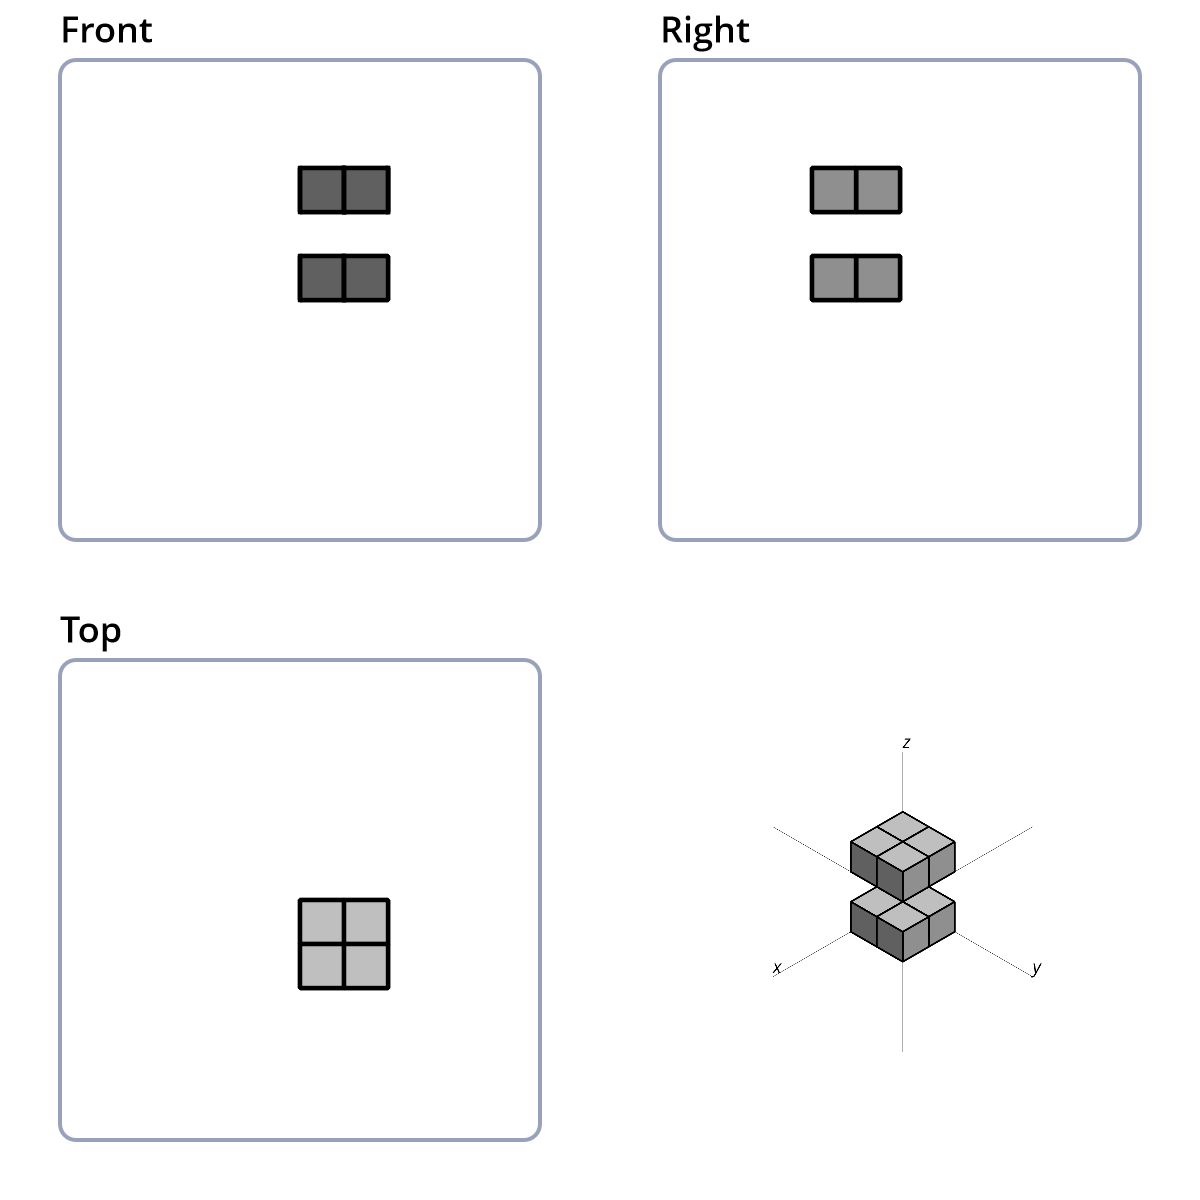
\includegraphics[scale=0.4]{iso_settings/puffer_1.png}
	\caption{Isometric of replicator-1.}
  \label{fig:iso-puffer-1}
\end{figure}

\subsubsection{Puffer trains}
When two of this puffer-2 (see figure~\ref{fig:iso-puffer-2}) frontally collide,
a glider-4 (see figure \ref{fig:iso-glider-4}) emerges.
\begin{figure}
	\centering
	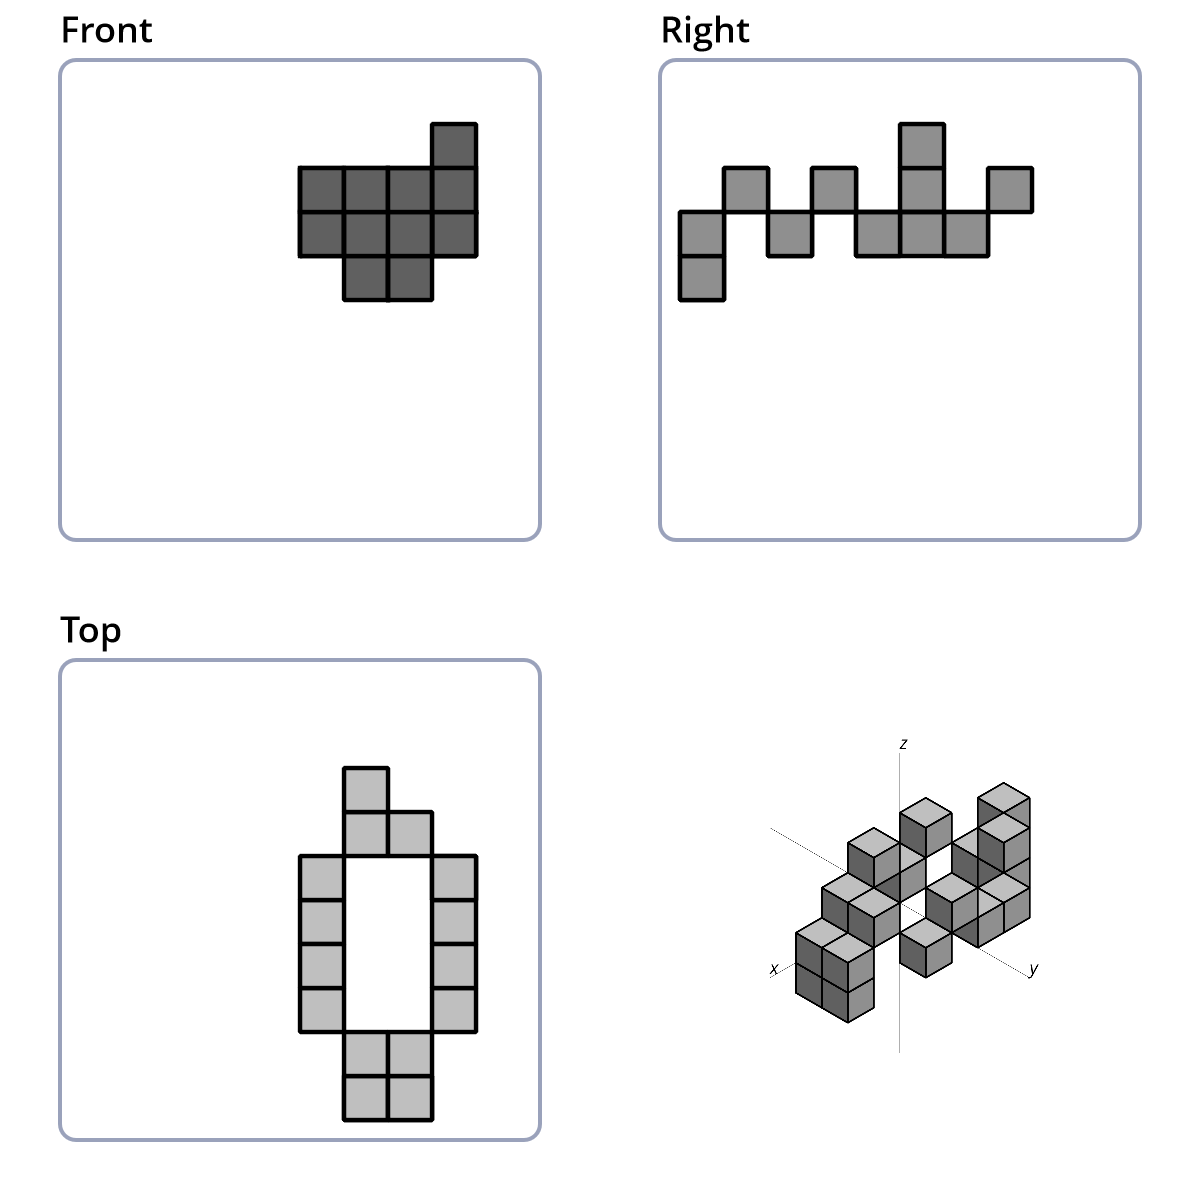
\includegraphics[scale=0.4]{iso_settings/puffer_2.png}
	\caption{Isometric of puffer-2.}
  \label{fig:iso-puffer-2}
\end{figure}
